% Author: Bernard Lampe

% Use the IEEE classes
\documentclass[journal]{IEEEtran}

% Packages
\usepackage[cmex10]{amsmath}
\usepackage{url}
\usepackage{cite}
\usepackage{graphicx}
\usepackage{subfig}
\usepackage{float}

% Start document
\begin{document}

% Paper title
\title{Computation of Rate-Distortion Function}

% Author
\author{Bernard~Lampe,~\IEEEmembership{Member,~IEEE}}

% The paper headers
\markboth{Computation of Rate-Distortion Function}
{Shell \MakeLowercase{\Lampe}: Computation of Rate-Distortion Function}

% Make the title area
\maketitle

\begin{abstract} Rate distortion theory is useful when computing the minimum, lossy coding rate of a random, ergodic source given a distortion measure. Lossy coding can be practically realized in lossy compression and transmission schemes where reconstruction fidelity is sacrificed to achieve lower bit rates. The theory allows one to compute the theoretical minimum bound of the coding rate given a permissible amount of distortion. In his 1972 paper, ``Computation of Channel Capacity and Rate-Distortion Functions'', Blahut formulated and published a practical algorithm which can compute these theoretical limits. In this analysis, we implement Blahut's algorithm and investigate the lower bound coding rate of a parameterized binomial random source using the Hamming distortion measure.
\end{abstract}

% Keywords
\begin{IEEEkeywords}
Blahut, Rate-Distortion, Hamming Matrix
\end{IEEEkeywords}

% Introduction with drop letter and first word capitalized.
\section{Introduction}
\IEEEPARstart{C}{laude} Shannon proved that the minimum coding rate at which a random, ergodic source can be compressed or transmitted in a lossless scheme is the source entropy. The coding rate used in this paper is number of bits per source symbol needed for compression or transmission. The source entropy is easily computed given the source probability distribution. A lossless scheme dictates that the source be reconstructed without error after compression or transmission. If we allow distortion (errors) in the reconstructed signal, we can achieve a smaller bit rate by sacrificing the signal fidelity. Given a random, ergodic source, rate distortion theory allows us to compute the minimum bit rate that is achievable under some bounded permissible distortion of the reconstruction. Practically, this is an extraordinarily useful theory when designing lossy compression or transmission algorithms \cite{shannon}.
\par Simply, rate distortion theory gives answers to two fundamental questions that arise when designing lossy coding schemes for a particular random source. One is, ``Given an allowed amount of distortion in the reconstructed signal, how many bits per source symbol do I have to use?'' It also addresses the converse question of, ``Given a particular coding rate, how much distortion will exist in the reconstructed signal?'' The theory does not take into account what the coding scheme is, it only tells you if it is achievable and what the theoretical lower bound is for all coding schemes given a particular source and distortion measure. The lower bound is specified by the rate distortion function denoted as \(R(D)\). A notional rate distortion curve is depicted below in figure \ref{fig:notional}. The gray region is the achievable coding rates at a particular distortion. The red curve is the lower bound. \cite{blahut}.

\begin{figure}[!h]
\centering
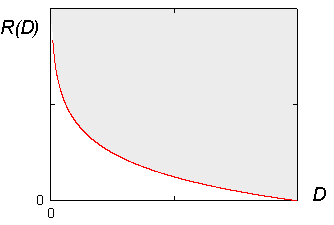
\includegraphics[width=3.1in]{../images/notional.png}
\caption{Notional Rate Distortion Function}
\label{fig:notional}
\end{figure}

\par There is a continuous debate about the definition of distortion measure. In this paper, we will use \(d(x,\hat{x})\) to denote the distortion error between the input \(x\) and the reconstruction output \(\hat{x}\). The most widely used distortion measure is the squared difference between the input and output as defined in equation \ref{eq:mse}. The expected value of this measure is known as the mean squared error. Another ubiquitous distortion measure is the Hamming or error probability matrix as defined in equation \ref{eq:hamming}. The Hamming measure defines a zero cost for correct reconstruction and a constant cost of \(1\) for errors. These distortion measures typically do not perform well on data which is meant for human perception such as music, images or video because they do not embody the aesthetics of the data. Also, aesthetics can be subjective from person to person. Therefore, the discussion of a suitable distortion measure will most likely continue well into the future. In this analysis, we have a discrete source and will be using the Hamming measure \cite{chang}.

\begin{equation}
\label{eq:mse}
d(x, \hat{x}) = (x - \hat{x})^2
\end{equation}

\begin{equation}
\label{eq:hamming}
 d(x, \hat{x}) =
  \begin{cases}
    1 & \quad \text{if } x \neq \hat{x} \\
    0 & \quad \text{if } x = \hat{x}
  \end{cases}
\end{equation}

\par A natural measure of total distortion for a particular sequence of input and output symbols is defined as the average of the distortion measure applied to the sequence as shown in equation \ref{eq:specDist}. When given a random source and the distortion measure, the expected value of the reconstruction distortion of any sequence of the source symbols is given in equation \ref{eq:expectedDist}, where \(J\) is the size of the input alphabet, \(K\) is the size of the output alphabet, \(p(x, \hat{x})\) is the joint probability between input and output and \(d(x, \hat{x})\) is defined above. Using Bayes rule we can transform the expectation of the distortion into equation \ref{eq:expectedDist2} where \(p(x)\) and \(d(x,\hat{x})\) is given as input. This formulation is useful because it explicitly shows the unknown quantity \(p(\hat{x}|x)\) which must be found during constrained optimization \cite[p.~301-310]{cover}.

\begin{equation}
\label{eq:specDist}
d(x^n, \hat{x}^n) = \frac{1}{n}\sum_{i=1}^{n}{d(x_i, \hat{x_i})}
\end{equation}

\begin{equation}
\label{eq:expectedDist}
E[d(x, \hat{x})] = \sum_{j=1}^{J}{\sum_{k=1}^{K}p(x_j, \hat{x_k})d(x_j, \hat{x_k})}
\end{equation}

\begin{equation}
\label{eq:expectedDist2}
E[d(x, \hat{x})] = \sum_{j=1}^{J}p(x_j)\left({\sum_{k=1}^{K}p(\hat{x_k}|x_j)d(x_j, \hat{x_k})}\right)
\end{equation}

\par The rate distortion function \(R(D)\) is defined as the minimum over the unknown parameter \(p(\hat{x}|x)\) of the mutual information between the input random source and output reconstructed signal given the constraint \(E[d(x,\hat{x})] \leq D\).The allowable distortion \(D\) is a given parameter and \(R\) can be computed analytically in specially cases. However, it is more often computed numerically using Blahut's algorithm. The definition of \(R\) is given in equation \ref{eq:R_D}. The unknown parameter \(p(\hat{x}|x)\) is the transition matrix of a compression or transmission channel. The same equation for \(R\) is restated in equations \ref{eq:R_D1} for clarity. Once \(R\) is computed for a particular source and distortion measure, the resulting curve can be used to answer the questions stated in the introduction.

\begin{equation}
\label{eq:R_D}
R(D) = \min_{p(\hat{x}|x):E[d(x, \hat{x})] < D} I(X;\hat{X})
\end{equation}

\begin{equation}
\label{eq:R_D1}
R(D) = \min_{p(\hat{x}|x):\sum_{j=1}^{J}p(x_j)\sum_{k=1}^{K}{p(\hat{x_k}|x_j)d(x_j,\hat{x_k})} < D} I(X;\hat{X})
\end{equation}

% Describe Blahut's Algorithm
\subsection{Blahut's Algorithm}
\par Blahut's algorithm is an iterative solution to equations \ref{eq:R_D} and \ref{eq:R_D1}. First Blahut cast the equation as a constrained optimization problem and formulated the solution using the well known technique of Lagrange multipliers. The new formulation of \(R(D)\) is in equation \ref{eq:lagrange} where \(D\) is defined in equation \ref{eq:lagrangeD}. With this pair of equations, \(D\) is no longer an input to the minimization. Given a particular Lagrange multiplier \(s\) we can compute both \(D\) and \(R(D)\) after we find the optimum \(p(\hat{x}|x)\). As it turns out, the \(s\) parameter is the slope of the curve at the computed \((D,R(D))\) point. Using this pair of equations, it is obvious that the optimization will have to be carried out for each point of the rate distortion curve given a particular \(s\).

\begin{multline}
\label{eq:lagrange}
R(D) = \min_{p(\hat{x}|x)}\biggl[\sum_{j=1}^{J}\sum_{k=1}^{K}p(x_j)p(\hat{x_k}|x_j)\log{\frac{p(\hat{x_k}|x_j)}{\sum_{j=1}^{J}p(x_j)p(\hat{x_k}|x_j)}} \\ - s\left(\sum_{j=1}^{J}\sum_{k=1}^{K}p(x_j)p(\hat{x_k}|x_j)d(x_j, \hat{x_k}) - D\right)\biggr]
\end{multline}

\begin{equation}
\label{eq:lagrangeD}
D = \sum_{j=1}^{J}\sum_{k=1}^{K} p(x_j)p(\hat{x_k}|x_j)^*d(x_j,\hat{x_k})
\end{equation}

\par Blahut uses the above Lagrange multiplier formulation to construct an iterative algorithm. First he defines the function \(F(p,p(\hat{x}|x),q)\) as in equation \ref{eq:F}. This leads to a recasting of the rate distortion function as a double minimization as specified in the set of equations \ref{eq:newR_D}, \ref{eq:newD}, \ref{eq:q_k} and \ref{eq:newp}. The algorithm proceeds with the source input probabilities \(p(x_j)\), a distortion measure \(d(x,\hat{x})\) and choice of Lagrange multiplier \(s\). Also a nominal output distribution \(q_k\) is assumed to set the initial condition of the iteration. In this analysis we assumed a uniform distribution of size \(K\). With these inputs the transition probabilities can be computed as in equation \ref{eq:newp}. This gives an estimate of \(p(\hat{x}|x)\) which can be then used to compute an updated estimate of \(q_k\) as in equation \ref{eq:q_k}. These two equations are iterated until they converge. Upon convergence, \(R(D)\) and \(D\) can be computed using the Lagrange multiplier as in equations \ref{eq:newR_D} and \ref{eq:newD}. This procedure gives a single point on the rate distortion curve. Multiple iterations can be run with varying values of \(s\) to compute a densely sampled discrete representation of the function. In practice, values of \(-10\) to \(0\) worked well and there was no discernible benefit to increasing the range past \(-20\) \cite{blahut}.

\begin{multline}
\label{eq:F}
F(p,p(x|\hat{x}), d(x, \hat{x})) = \sum_{j=1}^{J}\sum_{k=1}^{K}p(x_j)p(\hat{x_k}|x_j)\log{\frac{p(\hat{x_k}|x_j)}{q_k}} \\
- s\sum_{j=1}^{J}\sum_{k=1}^{K}p(x_j)p(\hat{x_k}|x_j)d(x_j,\hat{x_k})
\end{multline}

\begin{equation}
\label{eq:newR_D}
R(D) = sD + \min_{q}\min_{p(\hat{x}|x)}F(p, p(\hat{x}|x),q_k)
\end{equation}

\begin{equation}
\label{eq:newD}
D = \sum_{j=1}^{J}\sum_{k=1}^{K}p(x_j)p(\hat{x_k}|x_j)d(x_j,\hat{x_k})
\end{equation}

\begin{equation}
\label{eq:q_k}
q_k = \sum_{j=1}^{J}p(x_j)p(\hat{x_k}|x_j)
\end{equation}

\begin{equation}
\label{eq:newp}
p(\hat{x_k}|x_j) = \frac{q_ke^{sd(x_j,\hat{x_k})}}{\sum_{k=1}^{K}q_ke^{sd(x_j,\hat{x_k}})}
\end{equation}

\par We implemented Blahut's algorithm using Matlab. Also, we validated the algorithm performance by computing the rate distortion functions of three sources using different distortion measures. The sources were chosen such that the rate distortion curves can be computed analytically and such can be used to validate the numerical algorithm performance. First we used a Bernoulli random source and Hamming measure. For the second two examples we used a uniform source and an asymmetric then a symmetric distortion measure.

% Show results on Bernoulli source using hamming
\subsection{Bernoulli Source using Hamming Distortion}
\par The probability distribution for the Bernoulli random source is simply stated as \(p(x_0) = p\) and \(p(x_1) = 1-p\) where \(p\) is a distribution parameter bounded from \(0\leq p \leq1\). The Hamming distortion measure specified in equation \ref{eq:hamming} was use to compute the following curves. The analytically computed rate distortion curve is specified in equation \ref{eq:binaryAnalytical} where the \(H(X)\) denotes the entropy calculation. The rate distortion function was computed for multiple parameterized values of the input distribution from \(0.1\) until \(0.5\) at increments of \(0.1\). The plots of both the analytically and numerically derived curves are in figure \ref{fig:binaryAnalytical}. The blue curve represents the numerically derived function computed using our implementation of Blahut's algorithm. The red curves plotted are the analytically derived functions. As you can see these curves match very closely in every case and gives confidence in our implementation.

\begin{equation}
\label{eq:binaryAnalytical}
R(D) = 
  \begin{cases}
    H(p) - H(D) & \quad \text{if } 0\leq D\leq \min\{{p,1-p}\} \\
    0 & \quad \text{if } D \geq \min\{{p,1-p}\}
  \end{cases}
\end{equation}

\begin{figure}[!h]
\centering
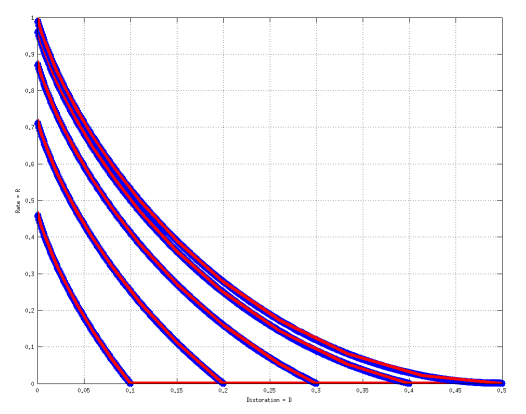
\includegraphics[width=3.1in]{../images/bernoulli.png}
\caption{\(R(D)\) of Bernoulli Random Sources using Hamming Distortion}
\label{fig:binaryAnalytical}
\end{figure}

% Show results on Uniform source with non-symmetric distortion matrix
\subsection{Uniform Source using Non-symmetric Distortion}
\par To further validate the Matlab implementation of Blahut's algorithm, another rate distortion function was computed for a non-symmetric coding scheme where the distortion matrix is not square. The source probability distribution was uniform with \(p(x_j) = 1/3\) and \(J=3\). The distortion measure used is specified in the matrix below in equation \ref{eq:asymmetric}. The analytically derived rate distortion function is given in equation \ref{eq:asymmetricRate} and is plotted in red in figure \ref{fig:asymmetric}. In the same figure, the numerically computed rate distortion is plotted in blue. The curves match very closely which gives confidence in the implementation when given a non-square distortion measure. This example is also interesting when observing the limits of the \(D\) axis. The minimum \(D\) is \(1\). This means that a coding scheme cannot be created that will result in zero distortion. Intuitively this follows from the fact that the compression or transmission channel will have \(3\) inputs and only \(2\) outputs meaning the source cannot be reproduced exactly. This implies only lossy schemes are possible.

\begin{equation}
\label{eq:asymmetric}
d(x,\hat{x}) = 
\begin{bmatrix}
1 & 2\\
1 & 1\\
2 & 1
\end{bmatrix}
\end{equation}

\begin{equation}
\label{eq:asymmetricRate}
R(D) = 
  \begin{cases}
    \frac{2}{3}(1-H(\frac{3}{2}(D-1)) & \quad \text{if } 1\leq D\leq \frac{4}{3} \\
    0 & \quad \text{if } D \geq \frac{4}{3}
  \end{cases}
\end{equation}

\begin{figure}[!h]
\centering
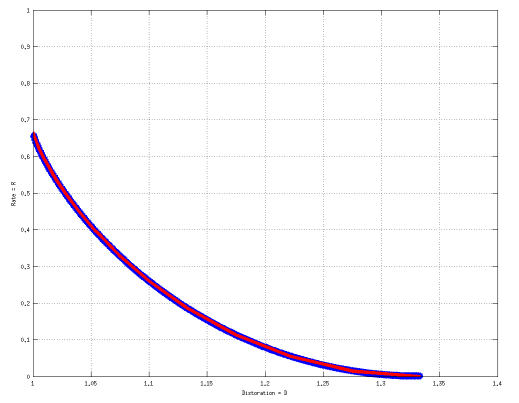
\includegraphics[width=3.1in]{../images/asymmetric.png}
\caption{\(R(D)\) of Uniform Source using Asymmetric Distortion}
\label{fig:asymmetric}
\end{figure}

% Show results on Uniform source with non-symmetric distortion matrix
\subsection{Uniform Source using Symmetric Distortion}
\par A final example was used to validate the Matlab implementation. This example uses a parameterized uniform random source with \(p(x_j)=\frac{1}{J}\) and symmetric Hamming distortion measure. The parameter specifies the discrete distribution size and distortion matrix size. The analytic solution is given in equation \ref{eq:symmetric} where \(J\) is the source distribution parameter. The plot of this function is given in figure \ref{fig:symmetric} in red. The plot shows many rate distortion functions for different sources for parameter \(J={2,3,4,5,6,7}\). As before, the blue curves represent the rate distortion functions computed via Blahut's numerical algorithm and match very closely. This gives extensive evidence for the correctness of the implementation.

\begin{equation}
\label{eq:symmetric}
R(D) = 
  \begin{cases}
    \log J - D\log(J-1) - H(D) & \quad \text{if } 0 \leq D \leq 1 - \frac{1}{J}\\
    0 & \quad \text{if } D \geq 1 - \frac{1}{J}
  \end{cases}
\end{equation}

\begin{figure}[!h]
\centering
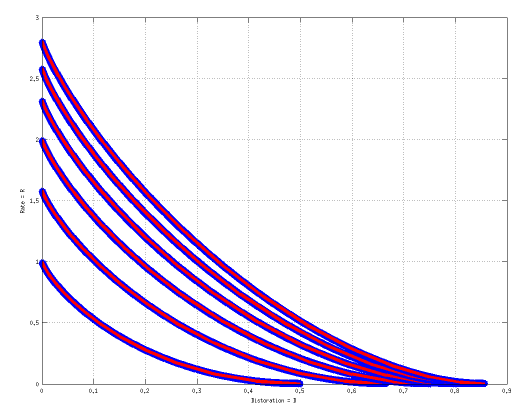
\includegraphics[width=3.1in]{../images/symmetric.png}
\caption{\(R(D)\) of Uniform Source using Symmetric Hamming Distortion}
\label{fig:symmetric}
\end{figure}

\section{Experiments}
\subsection{Binary Source Rate Distortion}
With the validated Matlab implementation, we explore the rate distortion function for a parameterized Binomial random source. The source is specified by equation \ref{eq:bernoulli} and is parameterized by the bounded coin-flipping trial probability \(0 \leq \theta \leq 1\) and size \(N\) representing the number of coin flips. Several of the input distribution curves are plotted in figure \ref{fig:binomialdist} using \(\theta={{0.1,0.2,0.3,0.4,0.5}}\) and \(N=50\). As expected, the distribution shifts to the middle of the range as \(\theta\) becomes closer to \(0.5\). Also, we plotted the input distribution for a constant \(\theta = 0.5\) and increasing \(N={ {10,20,30,40,50} }\). This plot was very similar to that in figure \ref{fig:binomialdist} as it showed centered binomial curves with increasing range.
\par When computing the \(R(D)\) curves for this parameterized source we used the Hamming distortion measure given in the introduction. Finally, we used the following source parameters \(\theta = {{0.1,0.2,0.3,0.4,0.5}}\) and size of \(N = {{10,20,30,40,50}}\) resulting in \(25\) rate distortion functions. The computed functions are in figures \ref{fig:theta_1}, \ref{fig:theta_2}, \ref{fig:theta_3}, \ref{fig:theta_4} and \ref{fig:theta_5}. The curves in a single figure all have the same input distribution parameter \(\theta\). Also, each figure contains \(5\) computed functions for increasing input distribution size parameter \(N\). All figures were plotted on the same absolute scale.
\par When assessing each figure individually the obvious trend is that while \(\theta\) stays constant and \(N\) increases, the coding rate \(R\) increases. This trend seems obvious when considering that the entropy of the larger sized input distributions is greater and therefore would require more bits per symbol even for the same allowable distortion. The trend of the increase appears logarithmic in that increasing the input distribution size increases the coding rate by smaller and smaller amounts.
\par When assessing the figures together another trend appears that while the \(N\) parameter is constant, increasing \(\theta\) increases the required coding rate given an allowable distortion. For example, examining figure \ref{fig:theta_1} where \(\theta=0.1\) shows the highest coding rate when \(D=0\) for \(N=50\) to be approximately \(3.1\). Upon comparing this with figure \ref{fig:theta_5} where \(\theta=0.5\) we see an increase to almost \(4\) bits per symbol when \(D=0\). This trend also appears to be logarithmic in nature as you increase the \(\theta\) parameter.
\par To help explain these trends, we plotted the source distribution entropy across the parameters \(\theta\) and \(N\) depicted in figure \ref{fig:3d} This plot shows that the source entropy \(H(X)\) is increasing in a logarithmic fashion when the input parameters \(\theta\) or \(N\) are increasing. Intuitively this makes sense as more bits per symbol would be needed as the variance of the distribution increases with \(\theta\) or the distribution size increases with \(N\).

\begin{equation}
\label{eq:bernoulli}
p(x|\theta) = {N \choose x}\theta^x(1-\theta)^{N-x} \text{  for  } x=1,\dots,N
\end{equation}

\begin{figure}[!h]
\centering
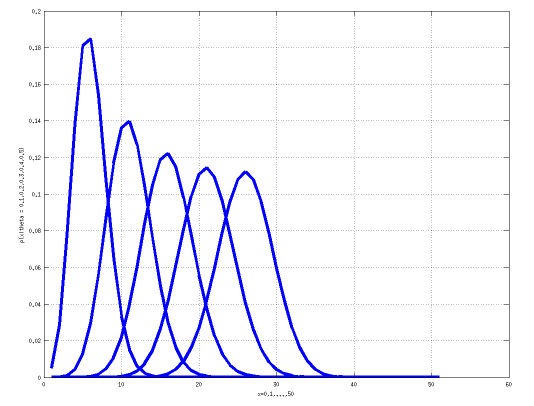
\includegraphics[width=3.1in]{../images/binomialdist.png}
\caption{Binomial PMF of Input Random Source \(N=50\)}
\label{fig:binomialdist}
\end{figure}


\begin{figure}[!h]
\centering
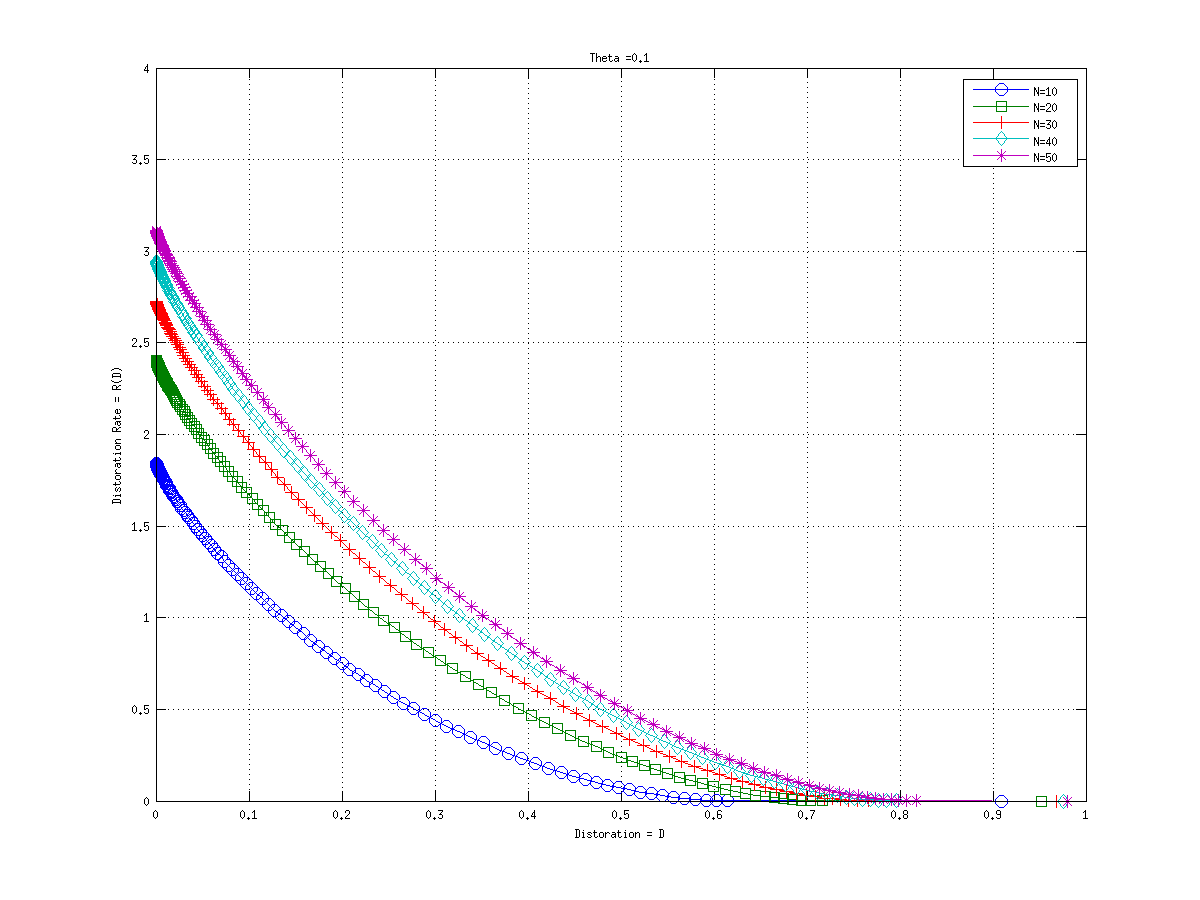
\includegraphics[width=3.1in]{../images/plot_1.png}
\caption{\(R(D)\) Curves for \(\theta=0.1\) and \(N={ {10,20,30,40,50} }\)}
\label{fig:theta_1}
\end{figure}

\begin{figure}[!h]
\centering
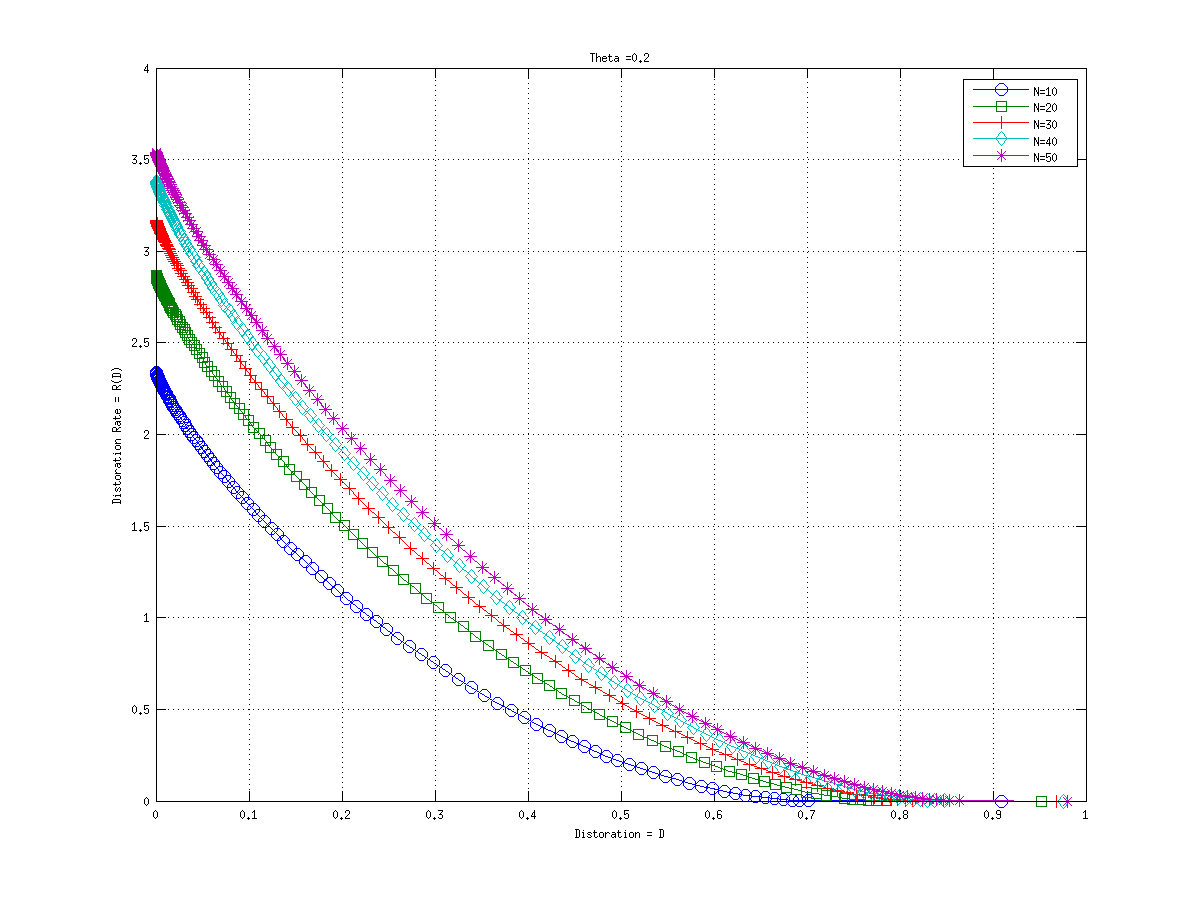
\includegraphics[width=3.1in]{../images/plot_2.png}
\caption{\(R(D)\) Curves for \(\theta=0.2\) and \(N={ {10,20,30,40,50} }\)}
\label{fig:theta_2}
\end{figure}

\begin{figure}[!h]
\centering
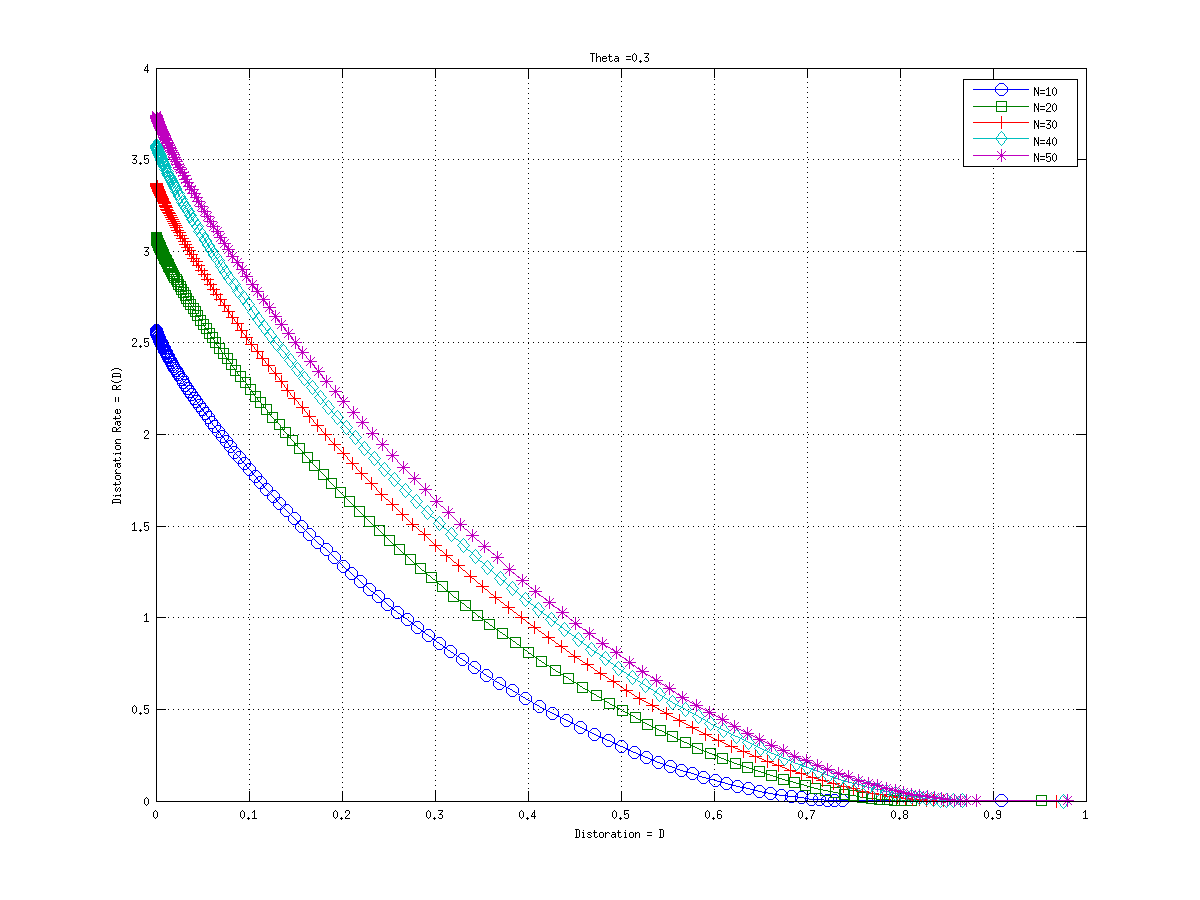
\includegraphics[width=3.1in]{../images/plot_3.png}
\caption{\(R(D)\) Curves for \(\theta=0.3\) and \(N={ {10,20,30,40,50} }\)}
\label{fig:theta_3}
\end{figure}

\begin{figure}[!h]
\centering
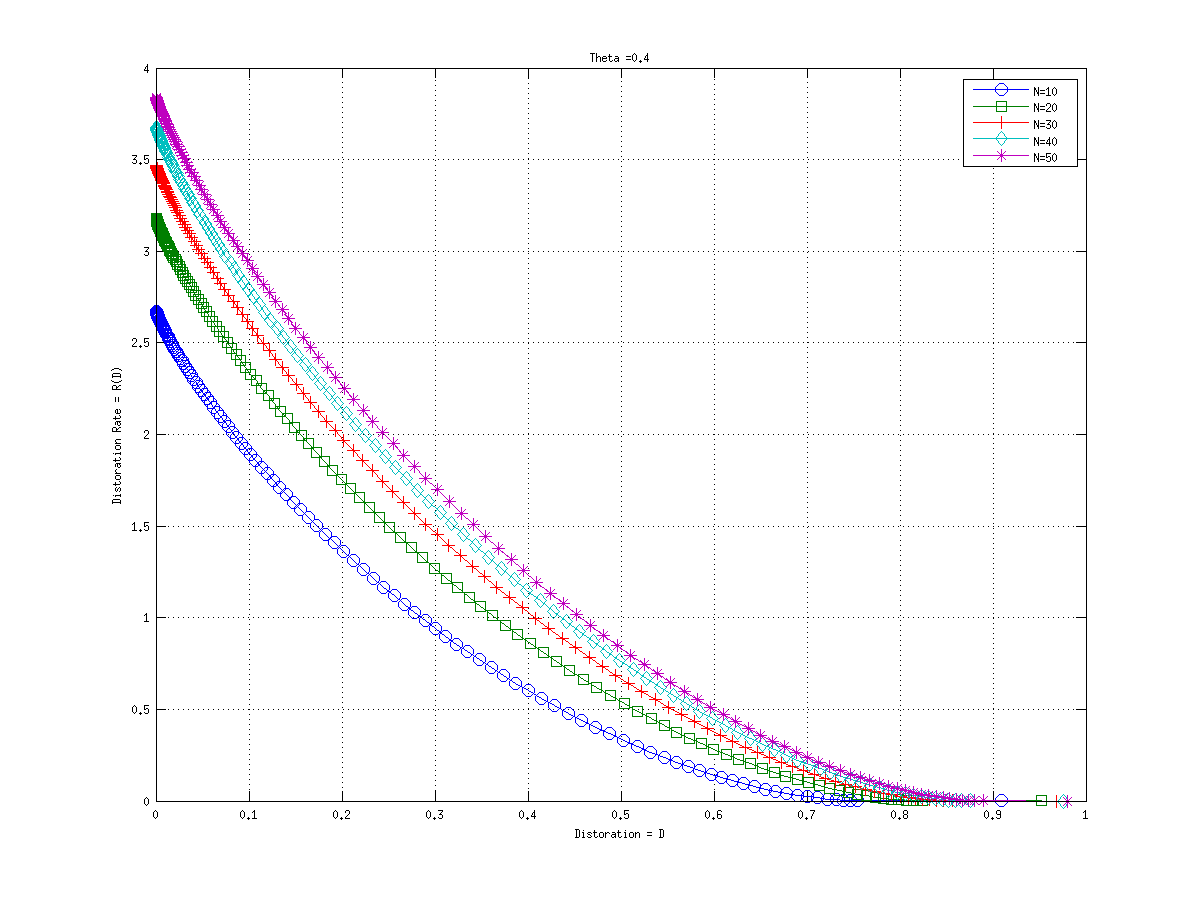
\includegraphics[width=3.1in]{../images/plot_4.png}
\caption{\(R(D)\) Curves for \(\theta=0.4\) and \(N={ {10,20,30,40,50} }\)}
\label{fig:theta_4}
\end{figure}

\begin{figure}[!h]
\centering
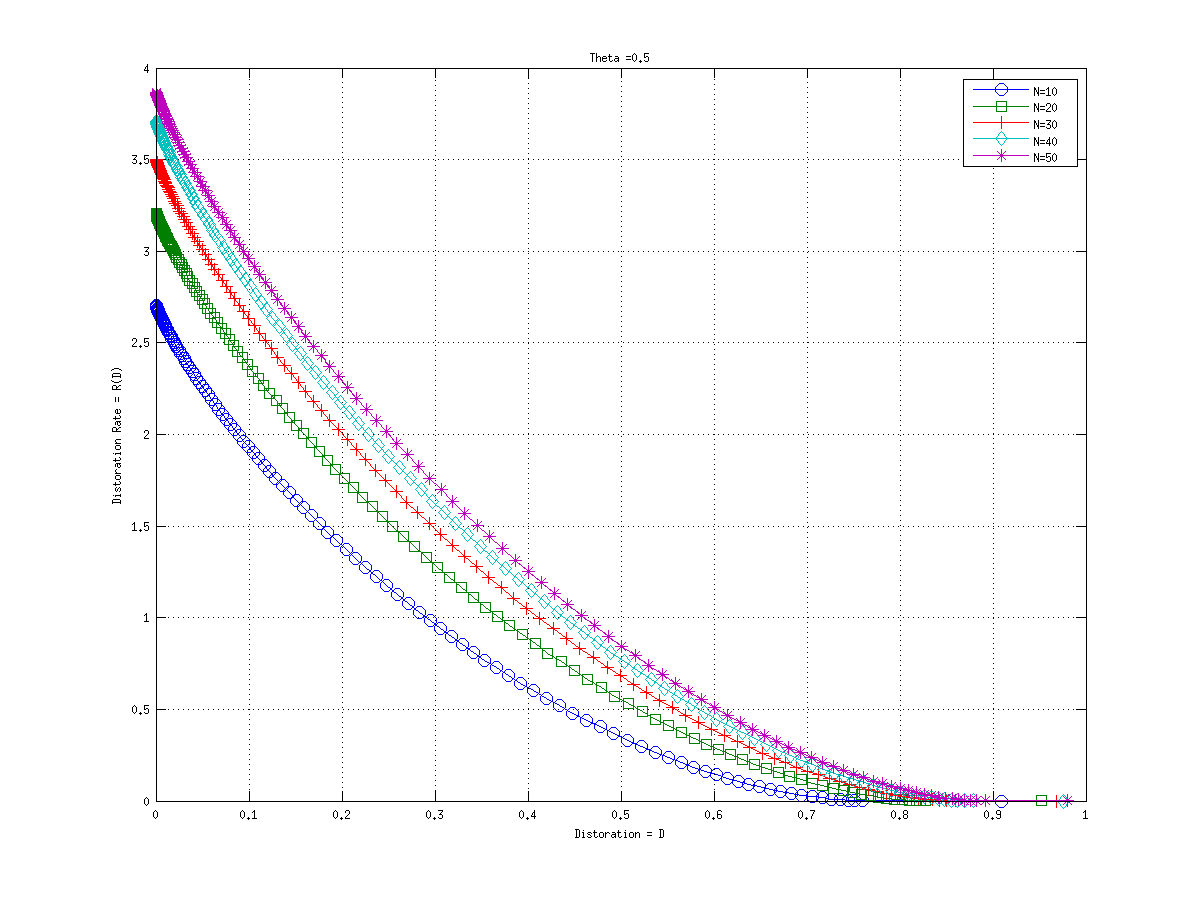
\includegraphics[width=3.1in]{../images/plot_5.png}
\caption{\(R(D)\) Curves for \(\theta=0.5\) and \(N={ {10,20,30,40,50} }\)}
\label{fig:theta_5}
\end{figure}

\begin{figure}[!h]
\centering
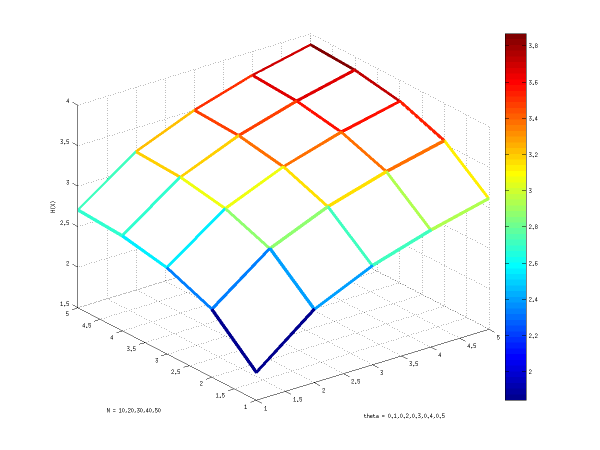
\includegraphics[width=3.1in]{../images/3d.png}
\caption{Mesh Plot of \(\theta,N,H(X)\) for Binomial Distribution}
\label{fig:3d}
\end{figure}

\section{Conclusion}
\par In this paper we have briefly introduced and summarized rate distortion theory and explained the utility when designing lossy compression or transmission schemes. We've also covered common distortion measures and restated the definition of the rate distortion functions. In addition, we detailed and implemented Blahut's numerical algorithm for computing rate distortion functions. We validated the performance of our algorithm with analytically computed examples and confirmed the code correctness. Finally, we explored the trends of the rate distortion functions of a parameterized binomial distribution. The two dominant trends of the rate distortion functions of the parameterized binomial distribution are a logarithmic increase in the required rate with increasing size or trial probability. This is due to the source entropy increasing as these parameters are increased. Intuitively more bits per symbol are required to compress or transmit the source if the size of the alphabet or probability variance of the input source increases. This holds in the lossless as well as the lossy case.

% References section
\nocite{*}
\bibliographystyle{plain}
\bibliography{./references}

% Biography
\begin{IEEEbiographynophoto}{Bernard Lampe}
(M'09) became an IEEE Member (M) in 2009 and received his bachelors of science degree from The University of Michigan in Ann Arbor, Michigan, USA in 2009.
\par Mr. Lampe is also a member of the American Society for Computing Machines (ACM) since 2009.
\end{IEEEbiographynophoto}

% End document
\end{document}

